 % -*- mode: LaTeX -*-
 % ... preamble ...
\documentclass[times,12pt,titlepage]{mstthesis}
\doublespacing
\usepackage{threeparttable}
\usepackage[final]{graphicx}
\usepackage{psfrag}
\usepackage{listings}
\usepackage{minted}
\usepackage[noprefix]{nomencl}
\usepackage{subcaption}
\usepackage{xr}
\makenomenclature
\renewcommand{\nomgroup}[1]{
   \ifthenelse{\equal{#1}{A}}{\medskip \item \textbf{Roman}}{}%
   \ifthenelse{\equal{#1}{G}}{\medskip \item \textbf{Greek}}{}%
   \ifthenelse{\equal{#1}{S}}{\medskip \item \textbf{Subscripts}}{}%
}
\usepackage[nopar]{lipsum} % ... provides dummy text ...

 % ... end preamble ...

\begin{document}

 % ... specify: ms or phd ...

\begin{ThesisTitlePage}{phd}

 % ... title page info ...

\author{\MakeUppercase{Edward T. Norris}}

\thesistitle{\MakeUppercase{Discrete Ordinates CT Organ Dose Simulator (DOCTORS)}}

\department{Nuclear Engineering}

 % ... thesis committee ...

\ThesisAdviser{Xin Liu}

 % If you have a co-advisor, enter the name in the
 % curly braces below and uncomment.
 % Otherwise, leave commented out.
 %\cothadviser{} % If you have 2 thesis advisers

\memberone{Ayodeji Alajo}
\membertwo{Hyoung Koo Lee}
\memberthree{Gary Mueller}
\memberfour{Fikret Ercal}
%\memberfive{Prandtl}

 % ... Graduation date - NOT your submission date ...
\graddate{2017}

\end{ThesisTitlePage}
 % ... copyright page - true|false ...

\copyrightyear{2017}
\ThesisCopyrightPage{true}

 % ... front matter - thesis abstract ...

\begin{ThesisAbstract}
This is the text for the abstract. Here, I explain what I did and how cool I am for doing it. Because I am awesome.
\end{ThesisAbstract}

 % ... front matter - thesis acknowledgements ...

\begin{ThesisAcknowledgment}
I would like to thank my adviser, Dr. Liu and all of the other graduate students for their continued support through my graduate career. I also appreciate the time spent by my committee members helping me identify problems and provide insight to solutions. 

I would also like to acknowledge the NRC for providing funding for my work. My work is supported by NRC grant NRC-HQ-13-G-38-0026.
\end{ThesisAcknowledgment}

\begin{ThesisFrontMatter}
\tableofcontents
\listoffigures
\listoftables
\listofsymbols
\end{ThesisFrontMatter}

\begin{ThesisBody}

 % ... introduction chapter ...
\ThesisBodyChapter{Introduction}%%
%% This is file `chapmin.tex',
%% generated with the docstrip utility.
%%
%% The original source files were:
%%
%% ths.dtx  (with options: `chapmin')
%% 
%% IMPORTANT NOTICE:
%% 
%% For the copyright see the source file.
%% 
%% Any modified versions of this file must be renamed
%% with new filenames distinct from chapmin.tex.
%% 
%% For distribution of the original source see the terms
%% for copying and modification in the file ths.dtx.
%% 
%% This generated file may be distributed as long as the
%% original source files, as listed above, are part of the
%% same distribution. (The sources need not necessarily be
%% in the same archive or directory.)


Computed tomography (CT) is becoming increasingly pervasive in medical diagnostics because improved algorithms are giving doctors more access to patient information. Increased information results in faster and more accurate diagnosis. However, the CT operation itself gives a radiation dose to the patient which carries some associated risk. A more detailed measure of that risk would help doctors make informed decisions regarding whether a CT scan is warannted, and if so, which type. This can also help doctors estimate spatial dose distribution to the patient to ensure no specific organ received more dose than permissible.

Currently, dose estimation relies on \textit{a priori} computation verified with a standardized benchmark. No methodology currently exists to verify that the dosimetry evaluation was accurate after the patient has undergone the procedure. This work proposes a methodology by which a patient's CT reconstruction is used to compute the dose received from the radiation beam.

Another, similar, application is dose estimation of patients receiving radiation therapy. Often, before the procedure, a time dependent, 4D CT scan of the patient is taken so that radiologists can account for breathing patterns during administration of the treatment. 

ESTIMATE. PHANTOM. CORRELATE.

BASED ON REFERENCE PHANTOM.

ADD FIGURE

Once the procedure (whether diagnostic or treatment) is completed, the dose distribution is assumed to follow the empirical model.

There are two primary methodologies available to provide the transport solution: Monte Carlo and deterministic methods. Monte Carlo has proven to be very slow in these areas. Further, the 3D Cartesian mesh generated from CT reconstruction is well suited to deterministic computation. 

This work forcuses on the discrete ordinates method and presents an implementation specially developed for dose estimation from a medical CT scan. 

Computational mesh from a sinogram. Reconstruction.
The DOCTORS code takes a computational reconstruction mesh of CT numbers, cross section data, and other parameters related to the solution methodology as input. The output is the collided and uncollided flux as well as the dose in each computational cell. These values can be compared to the empirical correlation results as a verification that the patient received an appropriate dose.

SHOULD BE FAST - GPU

USER INTERFACE

\endinput
%%
%% End of file `chapmin.tex'.

 % ... chapter ...
\ThesisBodyChapter{Literature Review}%%
%% This is file `chapbib.tex',
%% generated with the docstrip utility.
%%
%% The original source files were:
%%
%% ths.dtx  (with options: `chapmin,addbib')
%% 
%% IMPORTANT NOTICE:
%% 
%% For the copyright see the source file.
%% 
%% Any modified versions of this file must be renamed
%% with new filenames distinct from chapbib.tex.
%% 
%% For distribution of the original source see the terms
%% for copying and modification in the file ths.dtx.
%% 
%% This generated file may be distributed as long as the
%% original source files, as listed above, are part of the
%% same distribution. (The sources need not necessarily be
%% in the same archive or directory.)


 %% ... sample chapter ...

This section is the literature review. I do these things.

\section{Introduction}
Many different things are required.

\section{CT Dose Estimation}
How is this done now?

\section{CT Phantom Generation}
The CT phantom is populated with CT numbers, also known as Hounsfield numbers. These values are related to the attenuation coefficient of the material represented by the voxel.

Many authors have provided correlations that map the CT number to both a material and a density.

First ones.

The new guy provides 19 materials. The density is measured.

Two phantom datasets are used in this work.

\section{Discrete Ordinates}
Discrete ordinates are old.

Dort and Tort.

Denovo.

\section{GPU Acceleration}
GPUs are cool.

CUDA is cool.


\section{Section with \texttt{natbib} Citations}

This had been discussed previously by \citep{bullwinkle.1990} and
\citet{bullwinkle.1991}. \lipsum[22-25]


\endinput
%%
%% End of file `chapbib.tex'.

 % ... chapter ...
\ThesisBodyChapter{Methods}%%
%% Edward T. Norris
%% Discrete Ordinates Computed Tomography Organ Dose Simulator (DOCTORS)
%% 
%% === Methods ===
%%

This chapter summarizes the solution methodology employed by DOCTORS. The techniques used to compute the collided and uncollided fluxes are described in separate sections. After the flux solution methodology is explained, the methods used for source generation and flux-to-dose conversion are covered.

\section{Discrete Ordinate Methods}

The discrete ordinate solver computes the flux distribution inside the CT mesh given a source, physical geometry information, and other associated solver parameters such as quadrature and energy discretization. Discrete ordinates is a deterministic solution to the linear Boltzmann equation.

\subsection{The Boltzmann Equation}

The linear Boltzmann equation (LBE) is generally true of any particle given that outside forces (electromagnetic or gravitational) are either not present or negligible and particle-particle collisions are insignificant. Therefore, the LBE is generally not valid for charged particles or systems whose particle density is on the order of the medium they are traveling through. In such systems, particle-particle interactions may not be negligible.  

In general, the LBE is valid for multiplying media (such as neutrons passing through fuel in a reactor), but the variant considered in this work omits such terms since only photons in medical systems are of concern. Solutions to the LBE can also be used to solve criticality eigenvalue problems or to produce adjoint parameters for other codes. Such solutions are not considered in this work.

The steady state form of the LBE can be readily derived from simple intuition. In the steady state, particle production and removal must be equal. In any volume, three production mechanisms are present. Particles can (1) stream into the volume across a bounding surface, (2) inscatter from another energy-direction component of phase space, or (3) be produced directly by the external source. Three removal terms are also present, particles can (1) stream out of the volume of interest by crossing a bounding surface, (2) be absorbed and vanish entirely, or (3) outscatter to a energy-direction component of phase space other than the one of interest.

The downscatter and absorption removal terms are typically grouped together using
\begin{equation}
\Sigma_t = \Sigma_a + \Sigma_s
\end{equation}
where $\Sigma_t$, $\Sigma_a$, and $\Sigma_s$ are the macroscopic total, absorption, and scatter cross sections respectively. The removal of particles from interactions (scatter and absorption) per volume is then
\begin{equation}
\Sigma_t(\boldsymbol{r}, E) \psi(\boldsymbol{r}, E, \hat{\Omega})
\end{equation}
where $\psi$ is the angular flux. The production and removal streaming operators are combined as 
\begin{equation}
\hat{\Omega} \cdot \nabla \psi(\boldsymbol{r}, E, \hat{\Omega})
\end{equation}
and included as a removal term since the normal is defined pointing outward from the volume. The normal sign convention results in particles streaming out being positive and those streaming in becoming negative. 

The inscatter to a particular energy and direction is computed by integrating over all other energies and directions
\begin{equation}
\int_{4\pi}^{} \int_{0}^{\infty} \Sigma_s(\boldsymbol{r}, E' \rightarrow E, \hat{\Omega}' \rightarrow \hat{\Omega}) \psi(\boldsymbol{r}, E', \hat{\Omega}') dE' d\hat{\Omega}'.
\end{equation}
An external source $S$ produces particles per volume. Combining the removal terms on the left and the production terms on the right yields
\begin{equation} \label{eq:boltz}
\begin{split}
	&\left[ \hat{\Omega} \cdot \nabla + \Sigma_t(\boldsymbol{r}, E) \right]
	\psi(\boldsymbol{r}, E, \hat{\Omega}) = \\
	&\int_{4 \pi} \int_0^\infty \Sigma_s(\boldsymbol{r}, E' \rightarrow E, \hat{\Omega}' \rightarrow \hat{\Omega}) \psi(\boldsymbol{r}, E', \hat{\Omega}') dE' d\hat{\Omega}' + S(\boldsymbol{r}, E, \hat{\Omega})
\end{split}
\end{equation}
which is the LBE. The following sections show how Eq.~\ref{eq:boltz} is discretized and solved computationally.

\subsection{Angular Discretization}
The coordinate system used in DOCTORS is shown in Fig.~\ref{fig:coord_sys}. A discrete set of $N_a$ angles ($\Omega_{a}, \quad a = 0 \ldots N_a-1$) is selected to represent continuous directional space. Particles are transported only along these discrete directions from each voxel to adjacent voxels.

\begin{figure}[tb]
  \begin{center}
   \includegraphics[width=3.75in]{figs/coord_sys}
  \end{center}
  \caption{The coordinate system used in DOCTORS. Given an arbitrary direction, $\Omega$, $\mu$, $\eta$, and $\xi$ are its direction cosines with respect to the $x$, $y$, and $z$ axes respectively. $\varphi$ is the azimuthal angle (with respect to $x$ and the d $\theta$ is the polar angle (with respect to $z$).}
\label{fig:coord_sys}
\end{figure}

The rotation symmetrical quadrature is implemented in DOCTORS. From amongst many different quadrature sets, the rotation symmetrical quadratures were selected because they are easy to implement, rotationally symmetric, and the most commonly used in production discrete ordinate solvers [CITE] which enables simple, direct comparison to other solvers. Arbitrary quadratures are permissible in a plain text file supplied by the user enabling other quadratures.

THEORY AND MATH OF ANGLE/WEIGHT GENERATION?

To include a user defined quadrature, the plain text file should be formatted such that it contains four columns similar to Table~\ref{tab:quad_format} (without any headings). No checks are performed to ensure that octants are covered, this allows simple testing quadratures that utilize only a single direction to be used. Values for $\mu$, $\eta$, and $\xi$ do not necessarily need to add to unity as they will be automatically normalized by DOCTORS. Likewise, the weights will be normalized such that their summation is unity. However, user defined directions \textit{should not} be parallel to any major axis. Doing so may result in undefined behavior. Also, after normalization, no two rows should have identical values for $\mu$, $\eta$, and $\xi$ such as the last two rows of Table~\ref{tab:quad_interp}, nor may any weights be negative. The data in Table~\ref{tab:quad_format} would be read in and renormalized by DOCTORS. The normalized data would be identical to the data in Table~\ref{tab:quad_interp}.

Values are read in as a 32 bit IEEE-754 floating point number [CITE] which ensures seven significant digits. Significant digits beyond this will be truncated. Note that Table~\ref{tab:quad_interp} rounds four digits after the decimal.

\begin{table}[ht]
\caption{User Defined Quadrature Input}
\centering 
\begin{tabular}{c c c c}
\hline \hline   
$\mu$    & $\eta$ & $\xi$ & Weight\\ [0.5ex] 
\hline
1        & 0      & 0      & 1 \\
0.999    & 0.001  & 0.001  & 1 \\
1.0      & 1.0    & 1.0    & 1.3 \\
0.02198  & 0.2987 & .34520 & .02226 \\
.001     & .001   & .999   & 0.999 \\
-1       & 1      & -1     & .2 \\
-1.2     & 1.2    & -1.2   & 0.1 \\
-1        & 1     & -1     & .2 \\ [1ex]
\hline
\end{tabular}
\label{tab:quad_format}
\end{table}

\begin{table}[ht]
\caption{User Defined Quadrature Interpretation}
\centering 
\begin{tabular}{c c c c}
\hline \hline   
$\mu$    & $\eta$ & $\xi$ & Weight\\ [0.5ex] 
\hline
 1.0000  &  0.0000  &  0.0000  & 0.2074 \\
 1.0000  &  0.0010  &  0.0010  & 0.2074 \\
 0.5774  &  0.5774  &  0.5774  & 0.2696 \\
 0.0481  &  0.6536  &  0.7553  & 0.0207 \\
 0.5000  & -0.5000  &  0.7071  & 0.0046 \\
 0.5774  & -0.5774  & -0.5774  & 0.2072 \\
-0.5774  &  0.5774  & -0.5774  & 0.0415 \\
-0.5774  &  0.5774  & -0.5774  & 0.0415 \\ [1ex]
\hline
\end{tabular}
\label{tab:quad_interp}
\end{table}

A given direction, $\hat{\Omega}$, is determined by its three cosine components: 
\begin{equation} \label{eq:omega_cos}
\hat{\Omega} = \mu \hat{i} + \eta \hat{j} + \xi \hat{k}
\end{equation}
where $\hat{i}$, $\hat{j}$, and $\hat{k}$ are the unit directions in the $x$, $y$, and $z$ directions respectively. Therefore, any discrete direction $\hat{\Omega}_a$ can be expressed as $<\mu, \eta, \xi>$. The two forms will be used interchangeably.

Discretizing Eq.~\ref{eq:boltz} in angular space gives
\begin{equation} \label{eq:boltz_a}
\begin{split}
&\left[ \hat{\Omega}_a \cdot \nabla + \Sigma_t(\boldsymbol{r}, E) \right]
\psi_{a}(\boldsymbol{r}, E) = \\
&\sum_{a=0}^{N_a-1} \int_0^\infty \Sigma_{s, a, a'}(\boldsymbol{r}, E' \rightarrow E) \psi_{a'}(\boldsymbol{r}, E') dE' \omega_a + S_a(\boldsymbol{r}, E)
\end{split}
\end{equation}
where the subscript $a$ denotes the direction number and $\omega_a$ is a weight associated with that direction. The weights are designed with the angles such that once a discrete quadrature is selected, integration over continuous space becomes integration in discrete space approximated by
\begin{equation} \label{eq:disc_int}
\int_{4 \pi} f(\hat{\Omega}) d\hat{\Omega} \approx \sum_{a=0}^{N_a-1} f(\hat{\Omega}_a) \omega_a = 1.
\end{equation}

\subsection{Energy Discretization}

Continuous energy is discretized into $G$ groups indexed from 0 to $G-1$ as illustrated in Fig.~\ref{fig:energy_groups}. Therefore, Eq.~\ref{eq:boltz_a} becomes
\begin{equation} \label{eq:boltz_e}
\left[ \hat{\Omega}_a \cdot \nabla + \Sigma_t^g(\boldsymbol{r}) \right]
\psi_{a}^{g}(\boldsymbol{r}) = 
\sum_{a=0}^{N_a-1} \sum_{g'=0}^{G-1} \Sigma_{s, a, a'}^{g, g'}(\boldsymbol{r}) \psi_{a'}^{g'}(\boldsymbol{r}) \omega_a + S_a^g(\boldsymbol{r})
\end{equation}
where the group number is indexed by superscript $g$.

\begin{figure}[tb]
  \begin{center}
   \includegraphics[width=3.75in]{figs/energy_groups}
  \end{center}
  \caption{The energy grid structure used in DOCTORS. The highest energy group is group 0 and the lowest energy is group $G-1$.}
\label{fig:energy_groups}
\end{figure}

Once the energy group structure is selected, cross section data must be available. Group averaged cross section values from energy $E_1$ to $E_2$ are computed using Eq.~\ref{eq:groupxs} where $\sigma(E)$ is the continuous microscopic cross section. A weighting function, $f$, is used to weight some energies. The weighting function can be any of a number commonly used functions. The SCALE data libraries us a uniform function [CITE].
\begin{equation}\label{eq:groupxs}
\sigma_G = \frac{\int_{E_1}^{E_2}f(E')\sigma(E') dE'}{\int_{E_1}^{E_2} f(E') dE'}
\end{equation}

In photon based problems, upscatter is typically negligible [CITE]. By the time photons become low enough in energy to upscatter significantly, they are no longer of dosimetric concern. Removing upscatter reduces Eq.~\ref{eq:boltz_e} to
\begin{equation} \label{eq:boltz_e2}
\left[ \hat{\Omega}_a \cdot \nabla + \Sigma_t^g(\boldsymbol{r}) \right]
\psi_{a}^{g}(\boldsymbol{r}) = 
\sum_{a=0}^{N_a-1} \sum_{g'=g}^{G-1} \Sigma_{s, a, a'}^{g, g'}(\boldsymbol{r}) \psi_{a'}^{g'}(\boldsymbol{r}) \omega_a + S_a^g(\boldsymbol{r})
\end{equation}
which is very similar; only the starting point for the scatter summation changes. Computationally, though, the lack of upscatter makes a significant difference. The highest energy group can be solved independently of all those below it. Once that group is solved, the next group can also be solved and so forth. In the presence of upscatter, the highest group depends on the solution to all groups below it so all energy groups must be solved simultaneously.

The group structure cannot be arbitrarily selected by DOCOTRS, instead it is determined by the external cross section data file loaded by the user. The energy group structure should be selected appropriately for the problem. The cross sections currently included with DOCTORS are those available from the SCALE 6.2 distribution. Those cross sections are designed for light water reactor analysis and are not well suited to medical physics applications. This is currently one of the greatest limitations of DOCOTRS. The SCALE cross section data also contains neutron data which is useless for the CT dosimetry DOCTORS performs. More details of the cross section parsing and generation are included in Section~\ref{sec:xsparse} and~\ref{sec:xsgen} respectively.

\subsection{Spatial Discretization}

The problem domain is split into an evenly spaced Cartesian grid. Uniform grid spacing is not required by discrete ordinate methods though it is helpful [CITE], but is necessarily the case with CT voxel phantoms.

The problem domain for a CT voxel phantom is a regular, rectangular parallelepiped of dimension $D_x \times D_y \times D_z$, the values of which must be known based on the CT setup by the user. The mesh is partitioned into $N_x$, $N_y$, and $N_z$ evenly spaced bins along each major direction as shown in Fig.~\ref{fig:spatial_disc}. The total number of voxels, $N_V$ is easily computed from the number of bins in each major direction:
\begin{equation} \label{eq:n_v}
N_V = N_x N_y N_z.
\end{equation}
The length of a voxel along the $x$-direction is computed by 
\begin{equation} \label{eq:mesh_x}
\Delta x = \frac{D_x}{N_x}.
\end{equation}
Analogous equations apply in the $y$ and $z$ directions as well.

\begin{figure}[tb]
  \begin{center}
   \includegraphics[width=3.75in]{figs/spatial_disc}
  \end{center}
  \caption{The spatial mesh imposed on the problem domain.}
\label{fig:spatial_disc}
\end{figure}

Voxels can be indexed in one of two ways, either by their component indices or global index. Each voxel in the mesh has three components indices, one in each major direction, $i_x$, $i_y$, and $i_z$ that range from 0 to $N_x - 1$, $N_y - 1$, or $N_z-1$. However, this makes indexing cumbersome, so they are combined into a unique global index, $i$ using Eq.~\ref{eq:indx_flat}. In general, this is known as "flattening" a matrix into a one-dimensional vector. More details about the flattening implementation used in DOCTORS is given in Section~\ref{sec:flatten}.

\begin{equation} \label{eq:indx_flat}
i = i_x (N_z + N_y) + i_y N_z + i_z
\end{equation}

Using global indexing discussed, the fully discretized the steady state LBE given is
\begin{equation} \label{eq:boltz_i}
\left[ \hat{\Omega}_a \cdot \nabla + \Sigma_{t,i}^g \right]
\psi_{i,a}^{g} = 
\sum_{a=0}^{N_a-1} \sum_{g'=g}^{G-1} \Sigma_{s, i, a, a'}^{g, g'} \psi_{i, a'}^{g'} \omega_a + S_{i,a}^g
\end{equation}

\subsection{Solution}

To solve the fully discretized form of the Linear Boltzmann Equation given in Eq.~\ref{eq:boltz_i}, the gradient operator must first be computed numerically. Recall that $\Omega_a$ can be written in vector notation using its cosine components as defined in Eq.~\ref{eq:omega_cos}. Also recall the definition of the gradient:
\begin{equation} \label{eq:grad}
\nabla f(x, y, z) = \frac{\partial f(x, y, z)}{\partial x} \hat{i} + \frac{\partial f(x, y, z)}{\partial y} \hat{j} + \frac{\partial f(x, y, z)}{\partial z} \hat{k}.
\end{equation}
To a first order approximation, a partial derivative is computed as
\begin{equation} \label{eq:deriv_1}
\frac{\partial f(\zeta)}{\partial \zeta} \approx \frac{f(\zeta+\Delta \zeta/2) - f(\zeta + \Delta \zeta/2)}{\Delta \zeta}
\end{equation}
with respect to $\zeta$. Combining Eq.~\ref{eq:grad} and~\ref{eq:deriv_1}, the $\hat{\Omega} \cdot \nabla \psi$ term can be rewritten as:
\begin{equation} \label{eq:spatial_1}
\begin{split}
\Omega \cdot \nabla \psi 
& = <\mu, \eta, \xi> \cdot <\frac{\partial \psi}{\partial x}, \frac{\partial \psi}{\partial y}, \frac{\partial \psi}{\partial z}> \\
& =
\frac{\partial \psi}{\partial x}\mu + \frac{\partial \psi}{\partial y}\eta + \frac{\partial \psi}{\partial z}\xi \\
& \approx 
\frac{\psi(x + \Delta x/2, y, z) - \psi(x - \Delta x/2, y, z)}{\Delta x} \mu \\
&+ 
\frac{\psi(x, y + \Delta y/2, z) - \psi(x, y - \Delta y/2, z)}{\Delta y} \eta \\
&+ 
\frac{\psi(x, y, z + \Delta z/2) - \psi(x, y, z - \Delta z/2)}{\Delta z} \xi.
\end{split}
\end{equation}
The flux variables $\psi_{i,a,x,in}^g$, $\psi_{i,a,x,out}^g$, $\psi_{i,a,y,in}^g$, $\psi_{i,a,y,out}^g$, $\psi_{i,a,z,in}^g$, and $\psi_{i,a,z,out}^g$ are \textit{surface} averaged flux values while $\psi_{i,a}^{g}$ is a \textit{volume} averaged flux value.

The gradient is computed with respect to th edirection $\hat{\Omega}$, thus Eq.~\ref{eq:spatial_1} is valid only for the first octant ($\mu, \eta, xi > 0$). In other octants, a new gradient must be used. Rather than enumerating all eight variants, Eq.~\ref{eq:spatial_1} can be generalized to
\begin{equation} \label{eq:deriv_2}
\Omega \cdot \nabla \psi \approx 
\frac{\psi_{x,out} - \psi_{x,in}}{\Delta x} \mu + 
\frac{\psi_{y,out} - \psi_{y,in}}{\Delta y} \eta + 
\frac{\psi_{z,out} - \psi_{z,in}}{\Delta z} \xi
\end{equation}
where
\begin{equation}
\psi_{x,out} = 
\begin{cases}
\psi(x+\Delta x/2, y, z) \,, \quad \mu > 0 \\
\psi(x-\Delta x/2, y, z) \,, \quad \mu < 0
\end{cases}
\end{equation}
and
\begin{equation}
\psi_{x,in} = 
\begin{cases}
\psi(x-\Delta x/2, y, z) \,, \quad \mu > 0 \\
\psi(x+\Delta x/2, y, z) \,, \quad \mu < 0
\end{cases}
\end{equation}
and $\psi_{y,out}$, $\psi_{y,in}$, $\psi_{z,out}$, and $\psi_{z,in}$ are similarly defined but with respect to $\eta$ and $\xi$ respectively.

%\begin{figure}[tb]
%  \begin{center}
%   \includegraphics[width=3.75in]{figs/gradient}
%  \end{center}
%  \caption{The caption.}
%\label{fig:gradient}
%\end{figure}%

Using the generalized approximation given in Eq.~\ref{eq:deriv_2}, Eq.~\ref{eq:boltz_i} can be rewritten as
\begin{equation} \label{eq:boltz_i2}
\begin{split}
&\left[ 
\frac{\psi_{i,a,x,out}^g - \psi_{i,a,x,in}^g}{\Delta x} \mu + 
\frac{\psi_{i,a,y,out}^g - \psi_{i,a,y,in}^g}{\Delta y} \eta + 
\frac{\psi_{i,a,z,out}^g - \psi_{i,a,z,in}^g}{\Delta z} \xi
\right]
+ \Sigma_{t,i}^g \psi_{i,a}^{g} \\
& = 
\sum_{a=0}^{N_a-1} \sum_{g'=g}^{G-1} \Sigma_{s, i, a, a'}^{g, g'} \psi_{i, a'}^{g'} \omega_a + S_{i,a}^g.
\end{split}
\end{equation}

In order for the discretized LBE to be solved using Eq.~\ref{eq:boltz_i2}, both the incoming and outgoing flux must be known. Therefore, in order to compute the average flux in a cell, some relationship between the average flux and the outgoing surface fluxes must be known. These values can be related by any one of many different mechanisms, the most common of which is the diamond difference approximation.

\subsection{Diamond Difference Approximation}

The diamond difference approximation, relates the incoming and outgoing surface fluxes to the cell averaged flux. The cell averaged flux is assumed to be the average of any two opposite surface fluxes. This is assumed to be the case in all three spatial dimensions. This leads to:
\begin{equation} \label{eq:dd}
\begin{split}
\frac{\psi_{i,a,x,in}^g + \psi_{i,a,x,out}^g}{2} &= \psi_{i,a}^{g} \\
\frac{\psi_{i,a,y,in}^g + \psi_{i,a,y,out}^g}{2} &= \psi_{i,a}^{g} \\
\frac{\psi_{i,a,z,in}^g + \psi_{i,a,z,out}^g}{2} &= \psi_{i,a}^{g}.
\end{split}
\end{equation}
Multiplying both sides of Eq.~\ref{eq:dd} by 2 and subtracting twice the incoming surface flux from each yields:
\begin{equation} \label{eq:dd2}
\begin{split}
\psi_{i,a,x,out}^g - \psi_{i,a,x,in}^g &= 2\psi_{i,a}^{g} - 2\psi_{i,a,x,in}^g \\
\psi_{i,a,y,out}^g - \psi_{i,a,y,in}^g &= 2\psi_{i,a}^{g} - 2\psi_{i,a,y,in}^g \\
\psi_{i,a,z,out}^g - \psi_{i,a,z,in}^g &= 2\psi_{i,a}^{g} - 2\psi_{i,a,z,in}^g.
\end{split}
\end{equation}

The form of the left hand side of Eq.~\ref{eq:dd2} is the same as in Eq.~\ref{eq:boltz_i2}. This allows Eq.~\ref{eq:dd2} to be used to make a substitution in Eq.~\ref{eq:boltz_i2} that removes the dependence on the outgoing flux from discretized equation. After the substitution:
\begin{equation} \label{eq:boltz_i3}
\begin{split}
&\left[ 
\frac{2\psi_{i,a}^{g} - 2\psi_{i,a,x,in}^g}{\Delta x} \mu + 
\frac{2\psi_{i,a}^{g} - 2\psi_{i,a,y,in}^g}{\Delta y} \eta + 
\frac{2\psi_{i,a}^{g} - 2\psi_{i,a,z,in}^g}{\Delta z} \xi
\right]
+ \Sigma_{t,i}^g \psi_{i,a}^{g} \\
& = 
\sum_{a=0}^{N_a-1} \sum_{g'=g}^{G-1} \Sigma_{s, i, a, a'}^{g, g'} \psi_{i, a'}^{g'} \omega_a + S_{i,a}^g.
\end{split}
\end{equation}

Rearranging Eq.~\ref{eq:boltz_i3} to factor out the volume averaged flux term yields:
\begin{equation} \label{eq:boltz_i4}
\begin{split}
&\left[ 
\frac{2\psi_{i,a}^{g}}{\Delta x} \mu + 
\frac{2\psi_{i,a}^{g}}{\Delta y} \eta + 
\frac{2\psi_{i,a}^{g}}{\Delta z} \xi
\right] - 
\left[ 
\frac{2\psi_{i,a,x,in}^g}{\Delta x} \mu + 
\frac{2\psi_{i,a,y,in}^g}{\Delta y} \eta + 
\frac{2\psi_{i,a,z,in}^g}{\Delta z} \xi
\right]
+ \Sigma_{t,i}^g \psi_{i,a}^{g} \\
& = 
\sum_{a=0}^{N_a-1} \sum_{g'=g}^{G-1} \Sigma_{s, i, a, a'}^{g, g'} \psi_{i, a'}^{g'} \omega_a + S_{i,a}^g
\end{split}
\end{equation}
which can be directly solved for the volume averaged flux:
\begin{equation} \label{eq:boltz_i5}
\psi_{i,a}^{g} = 
\frac{
  \sum_{a=0}^{N_a-1} \sum_{g'=g}^{G-1} \Sigma_{s, i, a, a'}^{g, g'} \psi_{i,     a'}^{g'} \omega_a + 
  \left[ 
    \frac{2\psi_{i,a,x,in}^g}{\Delta x} \mu + 
    \frac{2\psi_{i,a,y,in}^g}{\Delta y} \eta + 
    \frac{2\psi_{i,a,z,in}^g}{\Delta z} \xi
  \right] + S_{i,a}^g
}{
  \frac{2\mu}{\Delta x}  + 
  \frac{2\eta}{\Delta y} + 
  \frac{2\xi}{\Delta z} + 
  \Sigma_{t,i}^g
}.
\end{equation}

The diamond difference approximation defined in Eq.~\ref{eq:dd} can also be rearranged to solve for each outgoing flux once the volume averaged flux is computed. The outgoing flux is:
\begin{equation} \label{eq:dd3}
\begin{split}
\psi_{i,a,x,out}^g &= 2\psi_{i,a}^{g} - \psi_{i,a,x,in}^g \\
\psi_{i,a,y,out}^g &= 2\psi_{i,a}^{g} - \psi_{i,a,y,in}^g \\
\psi_{i,a,z,out}^g &= 2\psi_{i,a}^{g} - \psi_{i,a,z,in}^g.
\end{split}
\end{equation}
The outgoing flux values are then used as the incoming flux values for subsequent voxels.

Repeatedly iteration Eq.~\ref{eq:boltz_i5} will eventually yield the solution to the flux distribution regardless of the initial guess. Choosing an accurate guess can greatly accelerate the code and guide convergence on a more accurate solution as discussed in more detail in Section~\ref{sec:uncol}. Either way, some metric must be used to determine when to stop the iteration process.

\subsection{Convergence Criteria}
The typical convergence criteria used to determine whether or to terminate further iteration is the maximum relative error from the $i-1^{th}$ iteration to the $i^{th}$ iteration given in Eq.~\ref{eq:conv} over the phase space $\mathbb{R}$. Once the relative error in the parameter of interest, $\phi$, is below some threshold, $\epsilon$, the iteration stops and the solution is considered converged.

\begin{equation}\label{eq:conv}
\max_{\mathbb{R}} \left\{ \frac{\phi_i - \phi_{i-1}}{\phi_i} \right\} < \epsilon
\end{equation}

In some problems, the convergence criteria given in Eq.~\ref{eq:conv} is not reached for many iterations. In these cases, terminating the solution early rather than waiting for full convergence is appropriate. This is enforced by a second criterial given by Eq.~\ref{eq:conv2}. Whenever the number of iterations, $i$, exceeds the total permissible number of iterations, $I$, the iteration is terminated.

\begin{equation}\label{eq:conv2}
i > I
\end{equation}

Under further investigation, the cause of the convergence failure that results in Eq.~\ref{eq:conv2} being exercised often stems from floating point error. The flux magnitude fluctuates wildly in regions of very flow flux, such as the gantry. In these regions, the relative uncertainty remains much higher than in regions with smoother flux distributions. 

FIGURE TO SHOW CONVERGENCE RATE.

In order to measure the uncertainty due to floating-point error, another convergence criteria was added. Rather than looking at the relative change from iteration to iteration, the total absolute change is measured:
\begin{equation}\label{eq:conv3}
\epsilon = \sum_{\mathbb{R}} |\phi_i - \phi_{i-1}|.
\end{equation}
The termination criteria is given by Eq.~\ref{eq:conv4}. Computation of a value for $\epsilon$ requires two previous iteration, thus this condition cannot be met until the third iteration and thereafter.

\begin{equation}\label{eq:conv4}
\epsilon_i > \epsilon_{i-1}
\end{equation}

\subsection{Anisotropy Treatment}

Scatter is assumed to be a function of only the scatter angle $\theta_s$ between the initial, $\hat{\Omega}_a$, and scattered, $\hat{\Omega}_{a'}$, directions. The cosine of the scatter angle, $\mu_s$ is related by 
\begin{equation} \label{eq:scat_cos}
\mu_s = \Omega_a \cdot \Omega_{a'} = \cos(\theta_s) \,, \quad 0 \leq \theta_s \leq \pi.
\end{equation}

\begin{figure}[tb]
  \begin{center}
   \includegraphics[width=3.75in]{figs/scat_ang}
  \end{center}
  \caption{The scatter angle. A photon (blue) at energy $E$ traveling in direction $\Omega$, hits a stationary atom (green) and scatters into a new direction $\Omega'$ with a new energy $E'$.}
\label{fig:scat_ang}
\end{figure}%

The data files containing the scatter cross sections are distributed using a Legendre polynomial expansion. The use of a Legendre expansion removes the dependence on the quadrature from the data. This allows any quadrature to work with any cross section dataset. A $l$-order Legendre polynomial is denoted by $P_l$. Details of the Legendre polynomials can be found in Appendix~\ref{appdx:leg}. The anisotropic scatter cross section is rewritten as a Legendre expansion as
\begin{equation} \label{eq:leg_1}
\Sigma_{s, i, a, a'}^{g, g'} = \sum_{l=0}^L \frac{2l+1}{4 \pi}\Sigma_{s, i, l}^{g, g'} P_l(\mu_s).
\end{equation}

\section{Uncollided Solution Methods}\label{sec:uncol}
One of the earliest problems with the discrete ordinate methods is the presence of ray effect. Ray effect arises due to the restriction of particle transport to a set of discrete directions. To illustrate ray effect, consider a point source streaming particles isotropically into vacuum. Since no scatter or absorption takes place in vacuum conditions, the particles can only stream and particles must be conserved. However, if particles are transported along a single discrete direction only as illustrated in Fig.~\ref{fig:rayeffect_ex} ($\hat{\Omega} = <\sqrt{2}/2, \sqrt{2}/2>$ in Fig.~\ref{rayeffect_ex} and~\ref{fig:rayeffect_comp}) the phenomena observed in Fig.~\ref{fig:rayeffect_comp} is observed. As the discretization becomes more refined, the isotropic source becomes more heavily biased in the $\hat{\Omega}$ direction. This phenomena is called ray effect and has been thoroughly studied by many \citep{ref:mathewsk} \citep{ref:tencerj}.

All particles must stream from one voxel to adjacent voxels. The streaming is considered (in 2D) along $<\sqrt{2}/2, \sqrt{2}/2>$ as shown in Fig.~\ref{fig:rayeffect_ex1}. All particles in the initial cell must stream outward into the two cells touching in the $\hat{\Omega}$ direction. The particles in each voxel split, half go to the voxel above and the other half travel to the right. This process is illustrated in Fig.~\ref{fig:rayeffect_ex}.

\begin{figure}
    \centering
    \begin{subfigure}[b]{0.2\textwidth}
        \includegraphics[width=\textwidth]{figs/rayeffect_ex1}
        \caption{}
        \label{fig:rayeffect_ex1}
    \end{subfigure}
    ~ 
    \begin{subfigure}[b]{0.2\textwidth}
        \includegraphics[width=\textwidth]{figs/rayeffect_ex2}
        \caption{}
        \label{fig:rayeffect_ex2}
    \end{subfigure}
    ~ 
    \begin{subfigure}[b]{0.2\textwidth}
        \includegraphics[width=\textwidth]{figs/rayeffect_ex3}
        \caption{}
        \label{fig:rayeffect_ex3}
    \end{subfigure}
    ~
    \begin{subfigure}[b]{0.2\textwidth}
        \includegraphics[width=\textwidth]{figs/rayeffect_ex4}
        \caption{}
        \label{fig:rayeffect_ex4}
    \end{subfigure}
    \caption{The process}\label{fig:rayeffect_ex}
\end{figure}

\begin{figure}
    \centering
    \begin{subfigure}[b]{0.45\textwidth}
        \includegraphics[width=\textwidth]{figs/rayeffect_iso4annot}
        \caption{}
        \label{fig:rayeffect_iso4annot}
    \end{subfigure}
    ~ 
    \begin{subfigure}[b]{0.45\textwidth}
        \includegraphics[width=\textwidth]{figs/rayeffect_beam4annot}
        \caption{}
        \label{fig:rayeffect_beam4annot}
    \end{subfigure}
    
    \begin{subfigure}[b]{0.45\textwidth}
        \includegraphics[width=\textwidth]{figs/rayeffect_iso12}
        \caption{}
        \label{fig:rayeffect_iso12}
    \end{subfigure}
    ~
    \begin{subfigure}[b]{0.45\textwidth}
        \includegraphics[width=\textwidth]{figs/rayeffect_beam12}
        \caption{}
        \label{fig:rayeffect_beam12}
    \end{subfigure}
    
    \begin{subfigure}[b]{0.45\textwidth}
        \includegraphics[width=\textwidth]{figs/rayeffect_iso500}
        \caption{}
        \label{fig:rayeffect_iso500}
    \end{subfigure}
    ~
    \begin{subfigure}[b]{0.45\textwidth}
        \includegraphics[width=\textwidth]{figs/rayeffect_beam500}
        \caption{}
        \label{fig:rayeffect_beam500}
    \end{subfigure}
    \caption{The ray effect artifact. The subfigures on the left (a, c, and e) show the correct solution modeled with $1/r^2$. The right subfigures (b, d, and f) show the corresponding solution with ray effect generated by the process described in Fig.~\ref{fig:rayeffect_ex}. The top row of subfigures uses 4 cells, the middle row uses 12, and the bottom row uses 500.}\label{fig:rayeffect_comp}
\end{figure}

The solution to prevent ray effect is to utilize an analytical uncollided source term. The full flux solution is split into two subproblems.
Equation~\ref{eq:boltz} is rewritten as two equations solving for the uncollided flux, $\psi_u$, and collided flux, $\psi_c$ independently:
\begin{equation} \label{eq:totflux}
\psi = \psi_u + \psi_c.
\end{equation}
Both $\psi_u$ and $\psi_c$ obey the LBE. The uncollided flux 
\begin{equation} \label{eq:unc}
\left[ \hat{\Omega} \cdot \nabla + \Sigma_t(\boldsymbol{r}, E) \right]
\psi_u(\boldsymbol{r}, E, \hat{\Omega}) =  S(\boldsymbol{r}, E, \hat{\Omega})
\end{equation}
has no scatter term since scattered particles are not considered in the uncollided flux. The lack of a scatter term makes the uncollided flux (whose analytical solution is derived shortly) computable with a raytracing algorithm. The uncollided flux is then used to compute the first collision source, $S_u$:
\begin{equation}\label{eq:uncsrc}
S_u = \int_{4\pi}^{} \int_{0}^{\infty} \Sigma_s(\boldsymbol{r}, E' \rightarrow E, \hat{\Omega}' \rightarrow \hat{\Omega}) \psi(\boldsymbol{r}, E', \hat{\Omega}') dE' d\hat{\Omega}'.
\end{equation}
which is then used to drive the collided flux in the same way the external source drives the uncollided flux distribution:
\begin{equation} \label{eq:col}
\begin{split}
	&\left[ \hat{\Omega} \cdot \nabla + \Sigma_t(\boldsymbol{r}, E) \right]
	\psi_c(\boldsymbol{r}, E, \hat{\Omega}) = \\
	&\int_{4 \pi} \int_0^\infty \Sigma_s(\boldsymbol{r}, E' \rightarrow E, \hat{\Omega}' \rightarrow \hat{\Omega}) \psi_c(\boldsymbol{r}, E', \hat{\Omega}') dE' d\hat{\Omega}' + S_{u}(\boldsymbol{r}, E, \hat{\Omega}).
\end{split}
\end{equation}
Substituting Eq.~\ref{eq:uncsrc} into $S_u$ in Eq.~\ref{eq:col} simplifies it to
\begin{equation} \label{eq:col2}
\begin{split}
	&\left[ \hat{\Omega} \cdot \nabla + \Sigma_t(\boldsymbol{r}, E) \right]
	\psi_c(\boldsymbol{r}, E, \hat{\Omega}) \\
	&=
	\int_{4 \pi} \int_0^\infty \Sigma_s(\boldsymbol{r}, E' \rightarrow E, \hat{\Omega}' \rightarrow \hat{\Omega}) \psi_c(\boldsymbol{r}, E', \hat{\Omega}') dE' d\hat{\Omega}' + \\
	&\int_{4\pi} \int_{0}^{\infty} 
\Sigma_s(\boldsymbol{r}, E' \rightarrow E, \hat{\Omega}' \rightarrow \hat{\Omega}) \psi_u(\boldsymbol{r}, E', \hat{\Omega}') 
dE' d\hat{\Omega}' \\
& = \int_{4 \pi} \int_{0}^{\infty} \Sigma_s(\boldsymbol{r}, E' \rightarrow E, \hat{\Omega}' \rightarrow \hat{\Omega}) \psi(\boldsymbol{r}, E', \hat{\Omega}') dE' d\hat{\Omega}'.
\end{split}
\end{equation}

A rigorous derivation for the uncollided flux is not provided in this work but can be obtained from [CITE]. Instead, an intuitive approach is used. First, consider an isotropic point source in a homogeneous media. The (scalar) flux well known to be
\begin{equation}
\varphi(r, E) = \frac{S(E) e^{-\mu(E) r}}{4 \pi r^2}
\end{equation}
where $S$ is the source strength, $\mu$ is the attenuation coefficient in the material, and $r$ is the distance traveled by the photon [CITE]. Expanding the problem to a full 3D model, the flux at $\boldsymbol{r}$ from a point source at $\boldsymbol{s}$ is
\begin{equation}\label{eq:isouncol}
\varphi(\boldsymbol{r}, E) = \frac{S(E) e^{-\mu(E) |\boldsymbol{r}-\boldsymbol{s}|}}{4 \pi |\boldsymbol{r}-\boldsymbol{s}|^2}.
\end{equation}
The only non-intuitive step is the introduction of anisotropy. The $4 \pi$ solid angle term in the denominator of Eq.~\ref{eq:isouncol} is generally expressed by
\begin{equation}\label{eq:anisonorm}
\int_{4 \pi}^{} \int_{0}^{\infty} S(E, \hat{\Omega}) dE d\hat{\Omega}
\end{equation}
but DOCTORS assumes $S$ is normalized such that the integral in Eq.~\ref{eq:anisonorm} is $4 \pi$. The flux is nonzero \textit{only} in the direction of travel, namely in the unit direction $\boldsymbol{r} - \boldsymbol{s}$. Therefore, a Kronecker delta function (defined in Eq.~\ref{eq:kronecker}) is used to produce the angular flux:
\begin{equation}\label{eq:uncsol}
\psi(\boldsymbol{r}, E, \hat{\Omega}) = \frac{S(E, \hat{\Omega}) e^{-\mu(E) |\boldsymbol{r}-\boldsymbol{s}|}}{4 \pi |\boldsymbol{r}-\boldsymbol{s}|^2} \delta \left( \hat{\Omega}, \frac{\boldsymbol{r} - \boldsymbol{s}}{|\boldsymbol{r} - \boldsymbol{s}|^2}\right).
\end{equation}

\begin{equation} \label{eq:kronecker}
\delta(\boldsymbol{A}, \boldsymbol{B}) = 
\begin{cases}
1 \,, \quad \mathrm{if} \ \boldsymbol{A}=\boldsymbol{B} \\
0 \,, \quad \mathrm{otherwise}
\end{cases}
\end{equation}

Equation~\ref{eq:uncsol} can be expanded to accomodate any number of spatially distributed sources of arbitrary directionality given in Eq.~\ref{eq:uncsol2} by integrating over the entire spatial domain, $V$
\begin{equation} \label{eq:uncsol2}
\psi_u(\boldsymbol{r}, E, \hat{\Omega}) = \iiint_{V}
S(\boldsymbol{s}, E, \hat{\Omega})
\frac{e^{-\sum_i \Sigma_{t,i} x_i}}{|\boldsymbol{r}-\boldsymbol{s}|^2}
\delta\left( \hat{\Omega}, \frac{\boldsymbol{r}-\boldsymbol{s}}{|\boldsymbol{r}-\boldsymbol{s}|^2}\right)
d \boldsymbol{s}.
\end{equation}


%\begin{equation} \label{eq:col3}
%\begin{split}
%	&\left[ \hat{\Omega} \cdot \nabla + \Sigma_t(\boldsymbol{r}, E) \right]
%	\psi_c(\boldsymbol{r}, E, \hat{\Omega}) = \\
%	&\int_{4 \pi} \int_0^\infty \Sigma_s(\boldsymbol{r}, E' \rightarrow E, %\hat{\Omega}' \rightarrow \hat{\Omega}) \psi(\boldsymbol{r}, E', %\hat{\Omega}') dE' d\hat{\Omega}'
%\end{split}
%\end{equation}

\section{Source Generation}
All photon transport problems considered in the DOCTORS code are ultimately driven by an external source, namely the medical equipment producing the photon beam. These sources can come in a variety of geometric shapes and energy spectra. Currently, DOCTORS has a number of built-in beam types available for analysis including point sources, fan beams, and cone beams. Fan beams and cone beams can be arranged about a phantom to produce an axial slice. Currently, helical paths are not supported, though they could be added with little additional effort. The geometry of fan beams and cone beams in DOCTORS is shown in Fig.~\ref{fig:shape}.

\begin{figure}
    \centering
    \begin{subfigure}[b]{.45 \textwidth}
        \includegraphics[width=\textwidth]{figs/shape_fanbeam}
        \caption{}
        \label{fig:shape_fanbeam}
    \end{subfigure}
    ~
    \begin{subfigure}[b]{.45 \textwidth}
        \includegraphics[width=\textwidth]{figs/shape_conebeam}
        \caption{}
        \label{fig:shape_conebeam}
    \end{subfigure}
    \caption{(a) The fanbeam is defined by $\theta$ in the polar coordinate and $\varphi$ azimuthally. (b) The cone beam is described only be $\theta$.}\label{fig:shape}
\end{figure}

\subsection{Point Source}
The simplest source implemented is an isotropic point source. This source is defined only by its position and energy distribution. Given a vector from the source to the center of the geometry, $\boldsymbol{s}$, and a vector from the source to the center of a cell, $\boldsymbol{c}$,the uncollided flux is computing using Eq.~\ref{eq:isouncol}. The collided flux is then computed using the discrete ordinate solution to the LBE given in Eq.~\ref{eq:col2}. The vectors are shown in Fig.~\ref{fig:phi}.

\begin{figure}[tb]
  \begin{center}
   \includegraphics[width=3.75in]{figs/phi}
  \end{center}
  \caption{Typical DOCTORS phantom geometry viewed axially with the phantom. The beam (gray) is centered on $\boldsymbol{s}$ and the vector from the source to the voxel of interest $\boldsymbol{c}$ is used to determine whether that voxel should be accepted or rejected. In the case of isotropic point sources, $\boldsymbol{s}$ is undefined.}
\label{fig:phi}
\end{figure}

\subsection{Fan Source}
In addition to the values defining a point source (position $\boldsymbol{s}$ and the energy distribution) a fan source is defined by two additional parameters, $\varphi$ and $\theta$ which describe the azimuthal and polar angles subtended by the fan beam respectively. Figure~\ref{fig:shape_fanbeam} shows $\varphi$ and $\theta$ with respect to the geometry setup. The raytracing algorithm used for the fan beam is identical to the point source raytracer except for one difference: before the raytracing is done, whether the ray falls within the fan beam is determined and any ray falling outside the fan beam is not traced, instead its uncollided flux is immediately set to zero. Some voxels are partially enclosed inside the beam which is not accounted for resulting in artifacts at the edges of the beam.

To determine whether a ray is accepted or rejected, the ray direction is first projected onto the $xy$ plane giving $<s_x, s_y, 0>$ and $<c_x, c_y, 0>$. Then the cosine of the angle between them, $\zeta_\varphi$, is computed using 
\begin{equation}\label{eq:phicos}
\cos(\zeta_\varphi) = \frac{<S_x, S_y, 0>}{\sqrt{S_x^2 + S_y^2}} \cdot \frac{<C_x, C_y, 0>}{\sqrt{C_x^2 + C_y^2}} = \frac{S_x C_x + S_y C_y}{\sqrt{S_x^2 + S_y^2} \sqrt{C_x^2 + C_y^2}}.
\end{equation}
Once $\zeta_\varphi$ is computed,
\begin{equation}\label{eq:phicoscon}
|\zeta_\varphi| < \frac{\varphi}{2}
\end{equation}
is evaluated. If the condition is met, the angle is accepted and raytraced normally, otherwise, it is rejected immediately.

Treatment for the $\theta$ variable is similar to that of $\varphi$ except the polar angle is required instead of the azimuthal angle. The polar angle of an arbitrary vector $\boldsymbol{\xi}$ can be computed using \begin{equation}\label{eq:thetacos}
\cos(\theta_\xi) = \frac{\xi_z}{\sqrt{\xi_z^2 + \xi_y^2 + \xi_z^2}}.
\end{equation}
This is used to compute the polar angle for both $\boldsymbol{s}$ and $\boldsymbol{c}$. The difference between the polar angles of the two vectors 
\begin{equation}\label{eq:thetacos2}
\zeta_\theta = \theta_s - \theta_c
\end{equation}
is used to evaluate
\begin{equation}\label{eq:thetacoscon}
|\zeta_\theta| < \frac{\theta}{2}.
\end{equation}
If the condition is not met, the ray is rejected and no raytrace is performed. Figure~\ref{fig:fan_rejection} shows a simple example demonstrating cases when a voxel would be accepted or rejected.

\begin{figure}[tb]
  \begin{center}
   \includegraphics[width=3.75in]{figs/fan_rejection}
  \end{center}
  \caption{The fan beam rejection. Voxels whose center lies outside the beam are rejected. This may lead to artifacts along the edges of the beam.}
\label{fig:fan_rejection}
\end{figure}

\subsection{Multi-fan Source}
The focal point about which the CT system rotates is assumed to be the center of the $xy$ plane and at the same $z$-elevation as the first user specified point. The focal spot defines the center of each fan beam.

\begin{figure}
    \centering
    \begin{subfigure}[b]{0.2\textwidth}
        \includegraphics[width=\textwidth]{figs/proj6}
        \caption{}
        \label{fig:proj6}
    \end{subfigure}
    ~ 
    \begin{subfigure}[b]{0.2\textwidth}
        \includegraphics[width=\textwidth]{figs/proj12}
        \caption{}
        \label{fig:proj12}
    \end{subfigure}
    ~ 
    \begin{subfigure}[b]{0.2\textwidth}
        \includegraphics[width=\textwidth]{figs/proj16}
        \caption{}
        \label{fig:proj16}
    \end{subfigure}
    ~
    \begin{subfigure}[b]{0.2\textwidth}
        \includegraphics[width=\textwidth]{figs/proj24}
        \caption{}
        \label{fig:proj24}
    \end{subfigure}
    \caption{Different numbers of fan beam projections ($N$). (a) $N = 6$. (b) $N = 12$. (c) $N = 16$. (d) $N = 24$.}\label{fig:fanproj}
\end{figure}

Rotation of an arbitrary point $(x,y)$ about the origin $\theta$ radians to a new position $(x', y')$ is performed by
\begin{equation}\label{eq:xp}
x' = x \cos \theta - y \sin \theta
\end{equation}
and
\begin{equation}\label{eq:yp}
y' = y \cos \theta + x \sin \theta.
\end{equation}

Rotation about an arbitrary point (namely the focal point), $(x_f, y_f)$ requires translating the system such that the focal point is at the origin, performing the rotation given in Eq.~\ref{eq:xp} and~\ref{eq:yp}, and then translating back to the original coordinates. This is done by
\begin{equation}\label{eq:xp2}
x' = (x-x_f) \cos \theta - (y-y_f) \sin \theta + x_f
\end{equation}
and
\begin{equation}\label{eq:yp2}
y' = (y - y_f) \cos \theta + (x - x_f) \sin \theta + y_f.
\end{equation}

\subsection{Cone Source and Multi-cone Source}
Cone sources are identical to fan beam sources except for the rejection criteria used to determine whether or not a voxel is inside the beam. The rejection criteria is a function of only a single parameter, $\theta$, the maximum permissible angle between the center of the beam, $\boldsymbol{s}$, and a ray toward the point of interest, $\boldsymbol{c}$.

The angle between $\boldsymbol{s}$ and $\boldsymbol{c}$ is
\begin{equation}\label{eq:zetacos}
\cos(\zeta) = \frac{<S_x, S_y, S_z>}{\sqrt{S_x^2 + S_y^2 + S_z^2}} \cdot \frac{<C_x, C_y, C_z>}{\sqrt{C_x^2 + C_y^2 + C_z^2}}
\end{equation}
which, if $\boldsymbol{s}$ and $\boldsymbol{c}$ are unit vectors, simplifies to
\begin{equation}\label{eq:zetacos}
\cos(\zeta) = S_x C_x + S_y C_y + S_z C_z.
\end{equation}
Once the angle is computed, the condition
\begin{equation}\label{eq:zetacon}
|\zeta| < \theta
\end{equation}
is evaluated to determine whether the ray is accepted or rejected.

\begin{figure}
    \centering
    \begin{subfigure}[b]{0.45\textwidth}
        \includegraphics[width=\textwidth]{figs/beamconexy}
        \caption{Cone xy}
        \label{fig:beamconexy}
    \end{subfigure}
    ~
    \begin{subfigure}[b]{0.45\textwidth}
        \includegraphics[width=\textwidth]{figs/beamfanxy}
        \caption{Fan xy}
        \label{fig:beamfanxy}
    \end{subfigure}

    \begin{subfigure}[b]{0.45\textwidth}
        \includegraphics[width=\textwidth]{figs/beamconeyz}
        \caption{Cone yz}
        \label{fig:beamconeyz}
    \end{subfigure}
    ~
    \begin{subfigure}[b]{0.45\textwidth}
        \includegraphics[width=\textwidth]{figs/beamfanyz}
        \caption{Fan yz}
        \label{fig:beamfanyz}
    \end{subfigure}
    
    \begin{subfigure}[b]{0.45\textwidth}
        \includegraphics[width=\textwidth]{figs/beamconexz}
        \caption{Cone xz}
        \label{fig:beamconexz}
    \end{subfigure}
    ~
    \begin{subfigure}[b]{0.45\textwidth}
        \includegraphics[width=\textwidth]{figs/beamfanxz}
        \caption{Fan xz}
        \label{fig:beamfanxz}
    \end{subfigure}
    \caption{The beam shapes.}\label{fig:beamfancone}
\end{figure}

\section{Dose Computation}
Dose can be computed in either one of two ways. The first way is to compute the fluence distribution and multiply by a fluence-to-dose conversion factor from ICRP 116 [CITE]. The second way to compute dose is to compute the energy deposition in each cell. In both methods, transport of secondary particles is neglected and all energy deposition is assumed to be local.

\subsection{Fluence-to-dose Conversion}

The publications of the ICRP include fluence-to-dose conversion factors for a reference phantom from various particle types and patient orientations. For CT systems, the rotationally symmetric (ROT) orientation is the most appropriate since the beam rotates about the patient. Figure~\ref{fig:icrp116_rotconv} shows the energy dependent fluence-to-dose conversions for the ROT orientation.

\begin{figure}[tb]
  \begin{center}
   \includegraphics[width=3.75in]{figs/icrp116_rotconv}
  \end{center}
  \caption{Fluence-to-dose conversion factors from ICRP 116 for photons.}
\label{fig:icrp116_rotconv}
\end{figure}

This methodology is very simplistic and can be computed quickly with no extra (memory) overhead. When DOCTORS finishes running, the scalar flux is multiplied by the conversion factor and summed over all energy groups:
\begin{equation}
D_i = \sum_{g=0}^{G-1} \varphi_i^g H^g
\end{equation}
where $H^g$ is the conversion factor for the $g^{th}$ group.

\subsection{Energy Deposition}

The alternative way to compute the dose is directly from the local energy deposition, $\mathcal{E}$, is by
\begin{equation}
\mathcal{E}_i = \sum_{g=0}^{G-1} \Sigma_{a,i}^g \varphi_i^g V_i \bar{E}^g F
\end{equation}
where $\bar{E}$ is the average energy (in MeV) of the $g^{th}$ group and $F$ is a unit conversion factor that converts MeV to Joules. The mass of the voxel, $M$ is then computed
\begin{equation}
M_i = \rho_i V_i G
\end{equation}
where $\rho_i$ is the density in g/cm$^3$ and G is a conversion factor to convert grams to kilograms. The dose in grays to the voxel is then
\begin{equation}
D_i = \frac{\mathcal{E}_i}{M_i} = \frac{\sum_{g=0}^{G-1} \Sigma_{a,i}^g \varphi_i^g \bar{E}^g F}{\rho_i G}.
\end{equation}

\endinput
%%
%% End of file `chapmin.tex'.


\ThesisBodyChapter{Implementation}%%
%% Edward T. Norris
%% Discrete Ordinates Computed Tomography Organ Dose Simulator (DOCTORS)
%% 
%% === Implementation ===
%%

This chapter covers the details of the implementation of the different components of the DOCTORS code base.

The code is available from the GitHub repository. At the time of this writing, the repository is located at \texttt{https://github.com/eNorris/thesis}.

The code is implemented in C++ and requires a C0x11 complianct compiler. The user interface is written using the Qt5 framework. GPU computation is performed via CUDA which must be compiled seperatly by Nvidia's proprietary compiler, \texttt{nvcc}.

\section{Vector Flattening}\label{sec:flatten}

Data is stored as \texttt{std::vector<>} objects.

Figure~\ref{fig:indx_ex} gives an example of the spatial indexing scheme using an $8 \times 8 \times 8$ mesh. The indicated voxel has $i_x$, $i_y$, and $i_z$ indices of 1, 5, and 6 respectively. Therefore, the index value of the highlighted voxel is $1 \times 8 \times 8 + 5 \times 8 + 6$ = 110. This flattening pattern continues to higher dimensional phase space to encompas energy and direction.

\begin{figure}[tb]
  \begin{center}
   \includegraphics[width=3.75in]{figs/indx_ex}
  \end{center}
  \caption{The indexing scheme.}
\label{fig:indx_ex}
\end{figure}

A variable that is dependent on $x$, $y$, $z$, $E$, and $\Omega$ would be written as $\phi(x, y, z, E, \Omega)$ would be discretized to $\phi(i_x, i_y, i_z, G, i_a)$. Rather than storing $\phi$ as a 5-dimensional matrix, $\phi$ is stored as a 1-dimensional vector of the same number of elements.

\section{Cross Section Parsing}\label{sec:xsparse}
AMPX cross sections are stored in a binary format. The binary file is split into a series of records. Each record contains a string of binary bytes between a four byte header and four byte footer. The header and footer are identical and, when interpreted as a signed four byte integer, give the size in words of the record. Each word is a 32-bit section (4~bytes) of binary data. An example record is shown in Fig.~\ref{fig:ampxbytes1}.

The data is stored in Big Endian format which must be converted to Little Endian for most Intel and AMD processors.  The endianess rearrangement is shown in Fig.~\ref{fig:ampxbytes2}. All records are one of 12 unique types. Each type of record is formatted and interpreted differently. For example, Type 1 contains general information about the data file such as the number of nuclides, number of energy groups, and a brief description. Type 2 records contains a list of floating-point numbers representing the energy group boundaries. Figure~\ref{fig:ampxbytes1} shows a Type 1 record. In the case of the header bytes given in Fig.~\ref{fig:ampxbytes1} and~\ref{fig:ampxbytes2}, the bytes correspond to the integer 440 which is the length in bytes of the record (not including the header or footer).

Each word of data is sequentially read, reordered, and converted to an apprpriately typed variable. Table~\ref{tab:reorder} shows the converstion for the record given in Fig.~\ref{fig:ampxbytes1}.

\begin{figure}[tb]
  \begin{center}
   \includegraphics[width=3.75in]{figs/ampxbytes1}
  \end{center}
  \caption{An example record parsed. The header and footer are identical and are the number of 32-bit words in the record.}
\label{fig:ampxbytes1}
\end{figure}

\begin{figure}[tb]
  \begin{center}
   \includegraphics[width=2.75in]{figs/ampxbytes2}
  \end{center}
  \caption{The byte reordering from Big Endian to Little Endian. Individual bits withing a byte are not rearranged, but the ordering of the four bytes withing a 32-bit word is reversed.}
\label{fig:ampxbytes2}
\end{figure}

\begin{table}[ht]
\caption{Byte Reordering}
\centering 
\begin{tabular}{l | c | c | c | l}
  \hline \hline   
  Word  & Big Endian & Little Endian & Interpreted & Notes\\ [0.5ex] % inserts table 
  \hline
  0   & B8 01 00 00 & 00 00 01 B8 & 440    & Header                    \\
  1   & 8B 69 00 00 & 00 00 69 8B & 27019  & ID                        \\
  2   & A4 01 00 00 & 00 00 01 A4 & 420    & Number of nuclides        \\
  ... &      ---    &      ---    &    --- & ---                       \\
  11  & 70 75 6F 43 & 43 6F 75 70 & "Coup" & First word of the title   \\
  12  & 20 64 65 6C & 6C 65 64 20 & "led " & Second word of the title  \\
  ... &     ---     &    ---      &  ---   & ---                       \\
  440 & 20 20 20 20 & 20 20 20 20 & "    " & 4 spaces ending the title \\
  441 & B8 01 00 00 & 00 00 01 B8 & 440    & Footer                    \\ 
  [1ex]      % [1ex] adds vertical space
  \hline
\end{tabular}
\label{table:reorder}
\end{table}

The header always reports the number of 8-bit bytes required to store the data. However, some data types, such as texttt{char}, are only one byte so each word represents multiple (4 in the case of \texttt{char}) distinct characters.

DOCTORS reads AMPX fromatted binary data files. Figure~\ref{fig:ampx} shows the data format of the overall file. 

The first entry in each nuclide entry is the directory record. The directory contains general information regarding the nuclide and information necessary to parse the proceeding records. Following the directory, Bondarenko data, resonance parameters, neutron data, and gamma production which are not of interest in photon only problems are read.

The penultimate record contains the average cross section data. This data is averaged over all energies and directions using Eq.~\ref{eq:groupxs}. The only data used in this section in DOCTORS is the total cross section values necessary for implementing the fully discretized form of the LBE given in Eq.~\ref{eq:boltz_i}.

The 2D data is stored in a special format optimized for scatter matrix data.

\begin{figure}
    \centering
    \begin{subfigure}[b]{0.45\textwidth}
        \includegraphics[width=\textwidth]{figs/ampx1}
        \caption{The AMPX file format}
        \label{fig:ampx1}
    \end{subfigure}
    ~
    \begin{subfigure}[b]{0.45\textwidth}
        \includegraphics[width=\textwidth]{figs/ampx2}
        \caption{The structure of each individual record.}
        \label{fig:ampx2}
    \end{subfigure}
    \caption{The format of the AMPX file. (a) The file contains a header, a list of directory records, energy group information and a list of nuclide entries. (b) Each nuclide entry contains multiple records; the two of concern in this work are the last two containing gamma data.}\label{fig:ampx}
\end{figure}

SHOW CARBON ELEMENTAL DATA

\section{Generation of Material Cross Section Data}\label{sec:xsgen}

Once the data is parsed, weighted combinations of elemental data is used to create material cross sections.

WATER EXAMPLE.

\begin{figure}
    \centering
    \begin{subfigure}[b]{0.45\textwidth}
        \includegraphics[width=\textwidth]{figs/airwaterxs2_19group}
        \caption{19 group data}
        \label{fig:airwaterxs2_19group}
    \end{subfigure}
    ~
    \begin{subfigure}[b]{0.45\textwidth}
        \includegraphics[width=\textwidth]{figs/airwaterxs2_47group}
        \caption{47 group data.}
        \label{fig:airwaterxs2_47group}
    \end{subfigure}
    \caption{Comparison of the group-averaged DOCTORS cross section data to continuous NIST data.}\label{fig:airwaterxs_group}
\end{figure}

\section{Qt5 Framework}\label{sec:qt}
The Qt5 framework was used for implementation of the user interface. Qt5 enables asynchronous calls through its ssignal/slot mechanism. A signal can be emitted which will execute all connected slots. Signals and slots can be connected manually by the user except for ones automatically generated by Qt. Qt prvides a user interface for building user interfaces. Components such a sbuttons, drop boxes, radio buttons, etc. are offered to the user. Qt makes extensive use of polymorphism. All user components inherit from the base \texttt{QWidget} class which inherits from \texttt{QObject}. Any class that utilizes the signal/sloot mechanism must extend the \texttt{QOjbect} class.

Listing~\ref{lst:sync1} gives a pseudocode snippet that has a long function that will block the user interface. A corresponding dequence diagram is given in Fig.~\ref{fig:sync1}. When the user interacts with the GUI, the writer object begins executing the \texttt{doWrite()} function. Until this function completes, the UI thread will be busy an dunable to handle additionaly user interaction or updates. This results in the GUI becoming unresponsive and potentially issuing a warning to the user from the operating system.

\begin{listing}
\begin{minted}[frame=lines,linenos]{python}
import numpy as np
def myfcn(hello,world):
   return hello*world
\end{minted}
\caption{Blah blah blah.}\label{lst:sync1}
\end{listing}

\begin{figure}[tb]
  \begin{center}
   \includegraphics[width=3.75in]{figs/writer_sync}
  \end{center}
  \caption{Sequence diagram for the synchronous call.}
\label{fig:sync1}
\end{figure}%

The code in Listing~\ref{lst:sync1} is updated to use the Qt signal/slot mechanism.

\begin{figure}[tb]
  \begin{center}
   \includegraphics[width=3.75in]{figs/writer_async}
  \end{center}
  \caption{Sequence diagram for the synchronous call.}
\label{fig:async1}
\end{figure}%

\section{Graphical User Interface}\label{sec:gui}

The GUI is cool. Lots of pictures of it.

\section{CUDA}\label{sec:cuda}
CUDA code is compoiled with the Nvidia complier nvcc. Qt uses the gcc compiler and its MOC generator for meta code. In order to connect CUDA code to the Qt MOC, the CUDA code is compiled by nvcc to produce a .o file. Qt then compiles all other files into corresponding.o files. The linker than automactically picks up all of the .o files gneerated by nvcc. The final result is an executable that has a Qt generarted user interface that can communicat with an Nvidia graphics card through the CUDA language.

The sweep through the mesh is different.

\begin{table}[ht]
\caption{Subsweep Indices}
\centering 
\begin{tabular}{l | c | c | c | c}
  \hline \hline   
  i  & ix & iy & iz & ix+iy+iz \\ [0.5ex] % inserts table 
  \hline
  0  & 4 & 0 & 0 & 4\\
  1  & 3 & 1 & 0 & 4\\
  2  & 3 & 0 & 1 & 4\\
  3  & 2 & 2 & 0 & 4\\
  4  & 2 & 1 & 1 & 4\\
  5  & 2 & 0 & 2 & 4\\
  6  & 1 & 3 & 0 & 4\\
  7  & 1 & 2 & 1 & 4\\
  8  & 1 & 1 & 2 & 4\\
  9  & 1 & 0 & 3 & 4\\
  10 & 0 & 4 & 0 & 4\\
  11 & 0 & 3 & 1 & 4\\
  12 & 0 & 2 & 2 & 4\\
  13 & 0 & 1 & 3 & 4\\
  14 & 0 & 0 & 4 & 4\\ [1ex]      % [1ex] adds vertical space
  \hline
\end{tabular}
\label{table:subsweep}
\end{table}

We first split the sweep process into $N_L$ subsweeps. For a $N_x \times N_x \times N_x$ mesh, the subsweep process is straightforward. Some of the initial subsweeps are shown for a $8 \times 8 \times 8$ mesh in Fig.~\ref{fig:subsweep_cube}. This is valid for any direction, $\hat{\Omega}$, for which all three of its direction cosines ($\mu$, $\xi$, and $\eta$) are positive.

\begin{figure}
    \centering
    \begin{subfigure}[b]{0.45\textwidth}
        \includegraphics[width=\textwidth]{figs/subsweep_cube1}
        \caption{Subsweep 0 ($S=0$)}
        \label{fig:subsweep_cube1}
    \end{subfigure}
    ~ %add desired spacing between images, e. g. ~, \quad, \qquad, \hfill etc. 
      %(or a blank line to force the subfigure onto a new line)
    \begin{subfigure}[b]{0.45\textwidth}
        \includegraphics[width=\textwidth]{figs/subsweep_cube2}
        \caption{Subsweep 1 ($S=1$)}
        \label{fig:subsweep_cube2}
    \end{subfigure}
    ~ %add desired spacing between images, e. g. ~, \quad, \qquad, \hfill etc. 
    %(or a blank line to force the subfigure onto a new line)
    \begin{subfigure}[b]{0.45\textwidth}
        \includegraphics[width=\textwidth]{figs/subsweep_cube3}
        \caption{Subsweep 6 ($S=6$)}
        \label{fig:subsweep_cube3}
    \end{subfigure}
    \begin{subfigure}[b]{0.45\textwidth}
        \includegraphics[width=\textwidth]{figs/subsweep_cube4}
        \caption{Subsweep 6 ($S=6$) with labels}
        \label{fig:subsweep_cube4}
    \end{subfigure}
    \caption{The progression of subsweeps throughout a sweep. Each subsweep must complete before those after it. Each voxel within a subsweep can be solved in parallel with all others in its subsweep.}\label{fig:subsweep_cube}
\end{figure}

In general, blah blah.

\begin{figure}
    \centering
    \begin{subfigure}[b]{0.2\textwidth}
        \includegraphics[width=\textwidth]{figs/subsweep_general1}
        \caption{$S=0$}
        \label{fig:subsweep_general1}
    \end{subfigure}
    ~ %add desired spacing between images, e. g. ~, \quad, \qquad, \hfill etc. 
      %(or a blank line to force the subfigure onto a new line)
    \begin{subfigure}[b]{0.2\textwidth}
        \includegraphics[width=\textwidth]{figs/subsweep_general2}
        \caption{$S=1$}
        \label{fig:subsweep_general2}
    \end{subfigure}
    ~ %add desired spacing between images, e. g. ~, \quad, \qquad, \hfill etc. 
    %(or a blank line to force the subfigure onto a new line)
    \begin{subfigure}[b]{0.2\textwidth}
        \includegraphics[width=\textwidth]{figs/subsweep_general3}
        \caption{$S=2$}
        \label{fig:subsweep_general3}
    \end{subfigure}
    \begin{subfigure}[b]{0.2\textwidth}
        \includegraphics[width=\textwidth]{figs/subsweep_general4}
        \caption{$S=3$}
        \label{fig:subsweep_general4}
    \end{subfigure}
    
    \begin{subfigure}[b]{0.2\textwidth}
        \includegraphics[width=\textwidth]{figs/subsweep_general5}
        \caption{$S=4$}
        \label{fig:subsweep_general5}
    \end{subfigure}
    ~ %add desired spacing between images, e. g. ~, \quad, \qquad, \hfill etc. 
      %(or a blank line to force the subfigure onto a new line)
    \begin{subfigure}[b]{0.2\textwidth}
        \includegraphics[width=\textwidth]{figs/subsweep_general6}
        \caption{$S=5$}
        \label{fig:subsweep_general6}
    \end{subfigure}
    ~ %add desired spacing between images, e. g. ~, \quad, \qquad, \hfill etc. 
    %(or a blank line to force the subfigure onto a new line)
    \begin{subfigure}[b]{0.2\textwidth}
        \includegraphics[width=\textwidth]{figs/subsweep_general7}
        \caption{$S=6$}
        \label{fig:subsweep_general7}
    \end{subfigure}
    \begin{subfigure}[b]{0.2\textwidth}
        \includegraphics[width=\textwidth]{figs/subsweep_general8}
        \caption{$S=7$}
        \label{fig:subsweep_general8}
    \end{subfigure}
    
    \begin{subfigure}[b]{0.2\textwidth}
        \includegraphics[width=\textwidth]{figs/subsweep_general9}
        \caption{$S=8$}
        \label{fig:subsweep_general9}
    \end{subfigure}
    ~ %add desired spacing between images, e. g. ~, \quad, \qquad, \hfill etc. 
      %(or a blank line to force the subfigure onto a new line)
    \begin{subfigure}[b]{0.2\textwidth}
        \includegraphics[width=\textwidth]{figs/subsweep_general10}
        \caption{$S=9$}
        \label{fig:subsweep_general10}
    \end{subfigure}
    ~ %add desired spacing between images, e. g. ~, \quad, \qquad, \hfill etc. 
    %(or a blank line to force the subfigure onto a new line)
    \begin{subfigure}[b]{0.2\textwidth}
        \includegraphics[width=\textwidth]{figs/subsweep_general11}
        \caption{$S=10$}
        \label{fig:subsweep_general11}
    \end{subfigure}
    \begin{subfigure}[b]{0.2\textwidth}
        \includegraphics[width=\textwidth]{figs/subsweep_general12}
        \caption{$S=11$}
        \label{fig:subsweep_general12}
    \end{subfigure}
    
    \begin{subfigure}[b]{0.2\textwidth}
        \includegraphics[width=\textwidth]{figs/subsweep_general13}
        \caption{$S=12$}
        \label{fig:subsweep_general13}
    \end{subfigure}
    ~ %add desired spacing between images, e. g. ~, \quad, \qquad, \hfill etc. 
      %(or a blank line to force the subfigure onto a new line)
    \begin{subfigure}[b]{0.2\textwidth}
        \includegraphics[width=\textwidth]{figs/subsweep_general14}
        \caption{$S=13$}
        \label{fig:subsweep_general14}
    \end{subfigure}
    ~ %add desired spacing between images, e. g. ~, \quad, \qquad, \hfill etc. 
    %(or a blank line to force the subfigure onto a new line)
    \begin{subfigure}[b]{0.2\textwidth}
        \includegraphics[width=\textwidth]{figs/subsweep_general15}
        \caption{$S=14$}
        \label{fig:subsweep_general15}
    \end{subfigure}
    \caption{The generalized subsweep.}\label{fig:subsweep_general}
\end{figure}

The number of parallel tasks, $P$, that can be done on subsweep $S$ of an $N_x \times N_y \times N_z$ mesh is given by Eq.~\ref{eq:taskspersub}.

\begin{equation}\label{eq:taskspersub}
P = C_S - L_x - L_y - L_z + G_{xy} + G_{yz} + G_{xz}
\end{equation}

\begin{equation}
C_S = \frac{(S+1)(S+2)}{2}
\end{equation}

\begin{equation}
L_x = \frac{d_x(d_x+1)}{2}
\end{equation}

\begin{equation}
L_y = \frac{d_y(d_y+1)}{2}
\end{equation}

\begin{equation}
L_z = \frac{d_z(d_z+1)}{2}
\end{equation}

\begin{equation}
G_{xy} = \frac{d_{xy}(d_{xy}+1)}{2}
\end{equation}

\begin{equation}
G_{yz} = \frac{d_{yz}(d_{yz}+1)}{2}
\end{equation}

\begin{equation}
G_{xz} = \frac{d_{xz}(d_{xz}+1)}{2}
\end{equation}

\begin{equation}
d_x = \max(S+1-N_x, 0)
\end{equation}

\begin{equation}
d_y = \max(S+1-N_y, 0)
\end{equation}

\begin{equation}
d_z = \max(S+1-N_z, 0)
\end{equation}

\begin{equation}
d_{xy} = \max(S+1-N_x - Ny, 0)
\end{equation}

\begin{equation}
d_{yz} = \max(S+1-N_y - Nz, 0)
\end{equation}

\begin{equation}
d_{xz} = \max(S+1-N_x - Nz, 0)
\end{equation}

Each voxel in a subsweep can be computed in parallel. Mathematically, the $i^{th}$ subsweep from all directions can be computed in parallel. However, in practice, this results in a race condition on the GPU hardware.


DELETE BELOW HERE.

The number of elements before the 4$^{th}$ level is 1 + 2 + 3 = 6. This is simply the sum of all integers less than the level number given by Eq.~\ref{eq:levelsum}. This is conincidentally the index of the first element of that level. However, there is a special case of $N_0 = 1$.

\begin{equation} \label{eq:levelsum}
N_L = \sum_{i=1}^{L} = \frac{L(L+1)}{2}
\end{equation}

Given an index, $i$, the level to which it belongs can be computed by substituting $i$ for $N_L$ in Eq.~\ref{eq:levelsum} and solving for $L$. The index value is then floored.

\begin{equation} \label{eq:levelquadratic}
i = \frac{L(L+1)}{2} \rightarrow L^2 + L - 2i = 0
\end{equation}

\begin{equation} \label{eq:levelquadsol1}
L = \left \lfloor{\frac{-1 \pm \sqrt{1+8i}}{2}} \right \rfloor
\end{equation}

Since the index must be a positive value, the $\pm$ sign can be removed from Eq.~\ref{eq:levelquadsol1} yielding Eq.~\ref{eq:levelquadsol2}

\begin{equation} \label{eq:levelquadsol2}
L = \left \lfloor{\frac{-1 + \sqrt{1+8i}}{2}} \right \rfloor
\end{equation}

The maximum index of any level in a the $N$ subsweep is $N$. Each subsweep adds an additional level. Therefore, the ix, iy, and iz indices can be computed using Eq.~\ref{eq:levelix},~\ref{eq:leveliy}, and~\ref{eq:leveliz} respectively.

\begin{equation} \label{eq:levelix}
ix = N - N_L
\end{equation}

\begin{equation} \label{eq:leveliy}
iy = L + N_L - i
\end{equation}

\begin{equation} \label{eq:leveliz}
iz = L + i - N_L
\end{equation}

\section{MCNP Generation}\label{sec:mcnpgen}
DOCTORS has the capability to generate MCNP6 input files from the CT mesh data and source specification provided by the user.

\section{Hardware}\label{sec:hardware}
For this work, a computer with an Intel i7-5960X 8 core (16 hyperthreads) processor with a base clock speed of 3.X GHz and an Nvidia Titan Z graphics card was used. Currently, if the problem requires more memory than is available on the GPU, the problem can still be solved, but much more time will be required to to copy overhead between the CPU and GPU. If the problem requires more memory than either the GPU or CPU can provide, an error is thrown and the simulation is not run.

CUDA is Nvidia only so AMD is not considered.

\endinput
%%
%% End of file `chapall.tex'.

 % ... conclusions chapter ...

\ThesisBodyChapter{Results}%%
%% This is file `chapmin.tex',
%% generated with the docstrip utility.
%%
%% The original source files were:
%%
%% ths.dtx  (with options: `chapmin')
%% 
%% IMPORTANT NOTICE:
%% 
%% For the copyright see the source file.
%% 
%% Any modified versions of this file must be renamed
%% with new filenames distinct from chapmin.tex.
%% 
%% For distribution of the original source see the terms
%% for copying and modification in the file ths.dtx.
%% 
%% This generated file may be distributed as long as the
%% original source files, as listed above, are part of the
%% same distribution. (The sources need not necessarily be
%% in the same archive or directory.)


\section{Preprocessing}
Two computational phantoms were used for verification of the DOCTORS code.

Some preprocessing was done to each phantom before it was used in DOCTORS to provide results.

The results from DOCTORS were compared to analagous results from MCNP6. The MCNP6 reference compared to is automatically generated by DOCTORS to guarantee that the geometry and source parameters are identical. This process is described in detail in Section~\ref{sec:mcnpgen}.

\subsection{Artifact Removal}
At the periphery of the computational mesh, artifacts can appear as a byproduct of the reconstruction algorithm used. Figure~\ref{fig:phantomWaterUnmodified} shows the artifacts in question in a $sy$ slice at the lowest ($z = 0$) level in the phantom. Two hundred sixty one (261) artifacts were detected in the phantom. To remove these artifacts, the CT number of any voxels whose CT number was greater than or equal to 65500 was set to 0. Figure~\ref{fig:phantomWaterModified} shows the same cross sectional plot after the artifacts are removed.

The water phantom in Fig.~\ref{fig:phantomWaterModified} can be broken into four regions: the water phantom, the container, the air, and the corner artifacts. The water phantom is the centermost region of the slice

\begin{figure}[tb]
  \begin{center}
   \includegraphics[width=3.75in]{figs/phantomWaterUnmodified}
  \end{center}
  \caption{The unmodified phantom. An $xy$ slice at $z$ index = 0.}
\label{fig:phantomWaterUnmodified}
\end{figure}

\begin{figure}[tb]
  \begin{center}
   \includegraphics[width=3.75in]{figs/phantomWaterModified}
  \end{center}
  \caption{The phantom after artifacts are removed. An $xy$ slice at $z$ index = 0.}
\label{fig:phantomWaterModified}
\end{figure}

\begin{table}[ht]
\caption{Water Regions}
\centering 
\begin{tabular}{l c r r}
\hline \hline   
Region    & CT Range & Voxels & Fraction (\%)\\ [0.5ex] 
\hline
Water     & $0 \leq x < 67$ & 1581199 & 37.70 \\
Container & $67 \leq x < 600$ & 81502 & 1.94 \\
Air       & $600 \leq x < 1080$ & 1650372  & 39.35 \\
Artifact  & $1080 \leq x < 65535$ & 881231 & 21.01 \\  [1ex]
\hline
\end{tabular}
\label{table:nonlin}
\end{table}

Once the artifacts are removed, the histogram is plotted. Figure~\ref{fig:waterHist} shows two versions of the water histogram, \ref{fig:waterHistLin} on a linear scale and \ref{fig:waterHistLog} on a logarithmic scale.

\begin{figure}
    \centering
    \begin{subfigure}[b]{0.45\textwidth}
        \includegraphics[width=\textwidth]{figs/waterHistogramLin2}
        \caption{Linear}
        \label{fig:waterHistLin}
    \end{subfigure}
    ~
    \begin{subfigure}[b]{0.45\textwidth}
        \includegraphics[width=\textwidth]{figs/waterHistogramLog}
        \caption{Logarithmic}
        \label{fig:waterHistLog}
    \end{subfigure}
    \caption{The histogram.}\label{fig:waterHist}
\end{figure}

\subsection{Gantry Handling}
The gantry is there.

\subsection{Geometry Simplification}
The original phantom data for both the water phantom and the liver phantom are $256\times256\times64$ meshes which result in 4,194,304 total voxels. Though MCNP6 is capable of running such a mesh, the overhead of loading the mesh into memory and initiating the Monte Carlo solver can take on the order of hours. Therefore, the benchmarks were run using a simplified geometry of $64\times64\times16$ which has only 65,536 voxels. The smaller files can run to completion of $10^9$ particles within two hours.

\section{Benchmark}

MCNP is good.

\section{Comparison}

They agree.


\endinput
%%
%% End of file `chapmin.tex'.
 
 
\ThesisBodyChapter{Conclusions}%%
%% This is file `chapmin.tex',
%% generated with the docstrip utility.
%%
%% The original source files were:
%%
%% ths.dtx  (with options: `chapmin')
%% 
%% IMPORTANT NOTICE:
%% 
%% For the copyright see the source file.
%% 
%% Any modified versions of this file must be renamed
%% with new filenames distinct from chapmin.tex.
%% 
%% For distribution of the original source see the terms
%% for copying and modification in the file ths.dtx.
%% 
%% This generated file may be distributed as long as the
%% original source files, as listed above, are part of the
%% same distribution. (The sources need not necessarily be
%% in the same archive or directory.)


 %% ... sample chapter ...

Conclusions.

\section{First conclusion}

I concluded many things.

\section{Future Work}

A number of simple modifications to DOCTORS could be made that would greatly increase the code's usability and robustness. One of these modifications, generation of more refined group structures, is not a change to DOCTORS \textit{per se} but rather a change in the input cross section data. The other changes are additions to DOCTORS that would add new capabilities to the software.

In addition to specific modifications, some additional, broader future goals can also be identified.

\subsection{Group Structure}

The cross section data currently used by DOCTORS are taken from SCALE6.2. While these cross sections have been found to be sufficient to produce flux distributions in medical CT imaging, a more refined group structure designed for medical applications would be worth investigation.

This work can be done using either NJOY [CITE] or the newly released AMPX [CITE] code. Either code has the capability to collapse an ENDF formatted data file into a group structure of the user's choosing in the format DOCTORS reads.



NJOY or AMPX.

\subsection{Temporal Extension}

Use 4D CT to do temporal stuff as well as spatial stuff.

\subsection{Multileaf Collimation}
Collimators!

\endinput
%%
%% End of file `chapmin.tex'.


\end{ThesisBody}
 % ... appendix - specify number of appendix chapters ...

\begin{ThesisAppendix}{two}
\ThesisAppendixChapter{Legendre Polynomials and Spherical Harmonics}%%
%% This is file `chapmin.tex',
%% generated with the docstrip utility.
%%
%% The original source files were:
%%
%% ths.dtx  (with options: `chapmin')
%% 
%% IMPORTANT NOTICE:
%% 
%% For the copyright see the source file.
%% 
%% Any modified versions of this file must be renamed
%% with new filenames distinct from chapmin.tex.
%% 
%% For distribution of the original source see the terms
%% for copying and modification in the file ths.dtx.
%% 
%% This generated file may be distributed as long as the
%% original source files, as listed above, are part of the
%% same distribution. (The sources need not necessarily be
%% in the same archive or directory.)


 %% ... sample chapter ...

This appendix covers the math for Legendre polynomials and spherical harmonics

\section{Legendre Polynomials}\label{appdx:leg}

They exist.

\subsection{Spherical Harmonics}

They also exist.

The real harmonics. The even/odd harmonics.

The addition theorem.

\endinput
%%
%% End of file `chapmin.tex'.


\ThesisAppendixChapter{Code Listings}%%
%% This is file `chapmin.tex',
%% generated with the docstrip utility.
%%
%% The original source files were:
%%
%% ths.dtx  (with options: `chapmin')
%% 
%% IMPORTANT NOTICE:
%% 
%% For the copyright see the source file.
%% 
%% Any modified versions of this file must be renamed
%% with new filenames distinct from chapmin.tex.
%% 
%% For distribution of the original source see the terms
%% for copying and modification in the file ths.dtx.
%% 
%% This generated file may be distributed as long as the
%% original source files, as listed above, are part of the
%% same distribution. (The sources need not necessarily be
%% in the same archive or directory.)


 %% ... sample chapter ...

This appendix covers different code listings.

\section{GUI}

This code does ...

\section{Raytracer}

\begin{listing}
%\begin{minted}[frame=lines,linenos,escapeinside=||,mathescape=true]{cpp}
\begin{minted}[frame=lines,linenos]{cpp}
// Given isx, isy, isz  source index
// Given sx, sy, sz source location
// Given node locations
// Given Deltas

// For every voxel
for iz0 = 0 .. Z-1
  for iy0 = 0 .. Y-1
    for ix0 = 0 .. X-1
    
      ir0 = ix0*NY*NZ + iy0*NZ + iz0
    
      // Start from the center of the cell containing the source
      x = xNodes[ir0] + Dx[isx]/2
      y = yNodes[ir0] + Dy[isy]/2
      z = zNodes[ir0] + Dz[isz]/2
      
      // End condition
      if ix0 == isx and iy0 == isy and iz0 == isz
        d = sqrt((x-sx)^2 + (y-sy)^2 + (z-sz)^2)
        for ie = 0 .. G-1
          mu = xsTot[ie, ir0] * atomDen[ir]
          uflux[ie, ir0] = S_0 * exp(-mu * d) / (4 * PI * d^2)
        SKIP TO NEXT CELL
        
      ix = ix0
      iy = iy0
      iz = iz0
      
      dx = sx - x
      dy = sy - y
      dz = sz - z
      
      d = sqrt((x-sx)^2 + (y-sy)^2 + (z-sz)^2)
      
      xcos = dx/d
      ycos = dy/d
      zcos = dz/d
      
      ixBound = NEXT X BOUNDARY INDEX
      iyBound = NEXT Y BOUNDARY INDEX
      izBound = NEXT Z BOUNDARY INDEX
      
      mfp[0 .. G-1] = 0
      
      exhausted = FALSE
      while not exhausted
        ir = ix*NY*NZ + iy*NZ + iz      
      
        tx = ...
        
        tmin = min(tx, ty, tz)
        dir = DIRECTION HIT
        
        for ie = 0 .. G-1
          mpf[ie] += tmin * xsTot[ir, ie] * atomDen[ir]
          
        if dir == X DIRECTION
          x = xNodes[ixBound]
          y += tmin*ycos
          z += tmin*zcos
          if xcos >= 0
            ix++
            ixBound++
          else
            ix--
            ixBound--
            
        if ix == ix0 and iy == iy0 and iz == iz0
          d = sqrt()
          for ie = 0 .. G-1
            mpf[ie] += d * xsTot[ie, ir] * atomDen[ir]
          exhausted = TRUE
          
      for ie = 0 .. G-1
        uflux[ir0, ie] = S0 * exp() / (4 * PI * d^2)

\end{minted}
\caption{Blah blah blah.}\label{lst:sync1}
\end{listing}

\section{Solver}

This code does ...

\endinput
%%
%% End of file `chapmin.tex'.


\ThesisAppendixChapter{Benchmark Results}%%
%% This is file `chapmin.tex',
%% generated with the docstrip utility.
%%
%% The original source files were:
%%
%% ths.dtx  (with options: `chapmin')
%% 
%% IMPORTANT NOTICE:
%% 
%% For the copyright see the source file.
%% 
%% Any modified versions of this file must be renamed
%% with new filenames distinct from chapmin.tex.
%% 
%% For distribution of the original source see the terms
%% for copying and modification in the file ths.dtx.
%% 
%% This generated file may be distributed as long as the
%% original source files, as listed above, are part of the
%% same distribution. (The sources need not necessarily be
%% in the same archive or directory.)


 %% ... sample chapter ...

This appendix covers details about the benchmarks that were not included.

\section{Benchmark}\label{sec:appc_benchmark}

The cone benchmark.

\begin{figure}
    \centering
    \begin{subfigure}[b]{0.45\textwidth}
        \includegraphics[width=\textwidth]{figs/bench_cone1_mc}
        \caption{The MCNP6 flux map.}
        \label{fig:bench_cone1_mc}
    \end{subfigure}
    ~
    \begin{subfigure}[b]{0.45\textwidth}
        \includegraphics[width=\textwidth]{figs/bench_cone1_mcunc}
        \caption{The MCNP6 uncertainty.}
        \label{fig:bench_cone1_mcunc}
    \end{subfigure}
    
    \begin{subfigure}[b]{0.45\textwidth}
        \includegraphics[width=\textwidth]{figs/bench_cone1_ray}
        \caption{The raytracer solution.}
        \label{fig:bench_cone1_ray}
    \end{subfigure}
    ~
    \begin{subfigure}[b]{0.45\textwidth}
        \includegraphics[width=\textwidth]{figs/bench_cone1_diff}
        \caption{The difference.}
        \label{fig:bench_cone1_diff}
    \end{subfigure}
    \caption{Comparison of the raytracer results to MCNP6 for the 10-20 MeV energy group.}\label{fig:waterHist}
\end{figure}

\section{Next benchmark}



\endinput
%%
%% End of file `chapmin.tex'.


\end{ThesisAppendix}

 % ... references - comma separated list of bib files ...

\begin{ThesisBibliography}{BIBLIOGRAPHY}
\bibliographystyle{plainnat}
\bibliography{refs}
\end{ThesisBibliography}

 % ... vita ...

\begin{Vita}
Edward Norris graduated from Missouri University of Science and Technology in 2013 with a B.S. in both nuclear engineering and computer science, he went on to pursue a M.S. in computer science and a PhD in nuclear engineering.

His PhD work was funded by a fellowship through the NRC.

Previously he has participated in four summer internships with Sandia National Laboratories. While there, he served in various capacities ranging from cyber defense to radiation detection and neutron scatter simulation.

Edward was awarded SOME AWARDS.

Edward was also an active member of the Nuclear Science Design Team at Missouri University of Science and Technology. While on the team he solved radiation transport problems to facilitate the dosimetry of an inertial electrostatic confintement fusion device being constructed.


\end{Vita}

\end{document}

